\documentclass[conference]{IEEEtran}
\usepackage[utf8]{inputenc}
\IEEEoverridecommandlockouts

\usepackage{cite}
\usepackage{amsmath,amssymb,amsfonts}
\usepackage{algorithmic}
\usepackage{algorithm}
\usepackage{graphicx}
\usepackage{textcomp}
\usepackage{xcolor}
\graphicspath{{./images/}}

\def\BibTeX{{\rm B\kern-.05em{\sc i\kern-.025em b}\kern-.08em
T\kern-.1667em\lower.7ex\hbox{E}\kern-.125emX}}

\title{MusicGen: A Variational Approach to Symbolic Music Generation}

\author{
    \IEEEauthorblockN{Anirudh Dambal}
    \IEEEauthorblockA{
        KLE Technological University\\
        Email: anirudh.dambal@example.com
    }
}

\begin{document}

\maketitle

\begin{abstract}
This paper presents MusicGen, a symbolic music generation framework using variational autoencoders (VAE). It leverages a piano roll representation of MIDI data to learn latent embeddings and synthesize novel sequences through probabilistic sampling and neural decoding.
\end{abstract}

% ==========================
% Methodology Section
% ==========================
\section{Methodology}
\label{sec:methodology}

\subsection{Data Preprocessing}
MIDI files are converted into a piano roll representation, a 2D binary matrix where rows correspond to MIDI pitches (0–127) and columns represent discrete time steps (e.g., 16th-note resolution). Each cell in the matrix is assigned a value of 1 if the note is active at that time step and 0 otherwise. The piano roll is segmented into fixed-length windows (e.g., 4-bar sequences) to standardize input dimensions for batch processing. This segmentation ensures temporal consistency and reduces computational complexity during training.

\subsection{VAE Architecture}
The variational autoencoder (VAE) consists of three primary components: an encoder, a stochastic sampling layer, and a decoder. The encoder maps input piano roll sequences to parameters of a latent space distribution (mean $\mu$ and log variance $\log\sigma^2$). The sampling layer generates latent vectors $z$ using the reparameterization trick:
\begin{equation}
    z = \mu + \sigma \odot \epsilon, \quad \epsilon \sim \mathcal{N}(0, 1),
\end{equation}
where $\sigma = \exp(0.5 \cdot \log\sigma^2)$. The decoder reconstructs the input sequence from the sampled latent vector $z$. The architecture employs convolutional layers in the encoder and transposed convolutional layers in the decoder to capture local temporal and pitch patterns.

\subsection{Loss Function}
The model optimizes a composite loss function combining reconstruction loss and Kullback-Leibler (KL) divergence. The reconstruction loss measures the binary cross-entropy between the input piano roll $X$ and the reconstructed output $\hat{X}$:
\begin{equation}
    \mathcal{L}_{\text{recon}} = -\frac{1}{N} \sum_{i=1}^N \left[ X_i \log \hat{X}_i + (1 - X_i) \log (1 - \hat{X}_i) \right],
\end{equation}
where $N$ is the total number of time-pitch pairs. The KL divergence regularizes the latent space to approximate a standard Gaussian distribution:
\begin{equation}
    \mathcal{L}_{\text{KL}} = \frac{1}{2} \sum_{j=1}^d \left( 1 + \log\sigma_j^2 - \mu_j^2 - \sigma_j^2 \right),
\end{equation}
where $d$ is the latent space dimension. The total loss is:
\begin{equation}
    \mathcal{L} = \mathcal{L}_{\text{recon}} + \beta \cdot \mathcal{L}_{\text{KL}},
\end{equation}
with $\beta$ controlling the regularization strength.

% ==========================
% Implementation Section
% ==========================
\section{Implementation}
\label{sec:implementation}

\subsection{Model Architecture}
\begin{figure}[h]
    \centering
    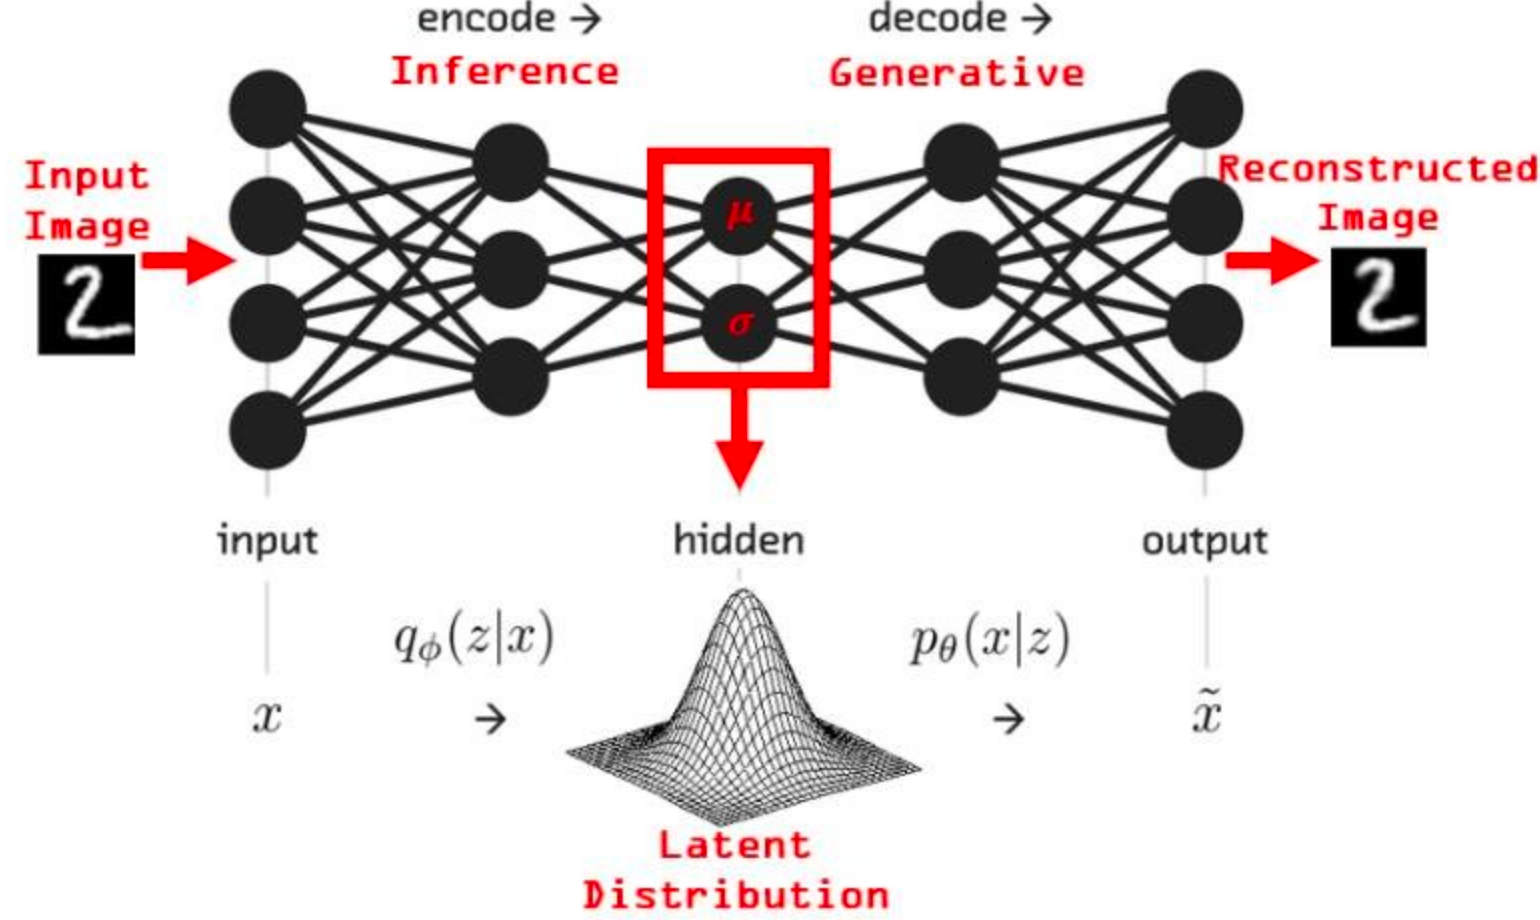
\includegraphics[width=\linewidth]{vae_architecture.png}
    \caption{Architecture of the variational autoencoder (VAE). The encoder maps input sequences to latent parameters $\mu$ and $\log\sigma^2$, the sampling layer generates $z$, and the decoder reconstructs the piano roll.}
    \label{fig:vae_arch}
\end{figure}

\subsection{Model Architecture}
The encoder uses two convolutional layers with $3 \times 3$ kernels and ReLU activation to extract hierarchical features from the input piano roll. The output is flattened and passed through dense layers to produce $\mu$ and $\log\sigma^2$. The decoder begins with a dense layer to project the latent vector $z$ into a tensor matching the encoder's output dimensions, followed by two transposed convolutional layers with $3 \times 3$ kernels to upsample the features. The final layer applies a sigmoid activation to generate probabilities in the range $[0, 1]$.


\subsection{Training Procedure}
Training utilizes the Adam optimizer with a learning rate of $10^{-4}$ and a batch size of 32. Early stopping monitors validation loss to prevent overfitting. Input sequences are normalized to binary values, and gradients are clipped to a maximum norm of 1.0 to stabilize training. The model is trained for 200 epochs, with $\beta$ annealed linearly from 0 to 1 during the first 50 epochs to prioritize reconstruction early in training.

\subsection{Music Generation}
Novel music sequences are generated by sampling latent vectors $z \sim \mathcal{N}(0, 1)$ and decoding them into piano rolls. Postprocessing includes thresholding (binarizing probabilities at 0.5) and temporal smoothing to remove transient notes shorter than 50 ms. The final piano roll is converted back to MIDI using note-on and note-off events with a fixed velocity (e.g., 100).

\end{document}
